\section{Incremental View Maintenance}\label{sec:relational}

Results in \secref{sec:streams} and~\secref{sec:incremental}
apply to streams of arbitrary group values.  In this
section we turn our attention to using these results in the context of 
relational view maintenance.  As explained in the introduction, we want to
efficiently compute the incremental version of any relational query $Q$
that updates a database view.

However, we face a technical problem: the $\I$ and $\D$ operators were
defined on abelian groups, and relational databases in general are 
not abelian groups, since they operate on sets.  Fortunately, 
there is a well-known tool in the database literature
which converts set operations into group operations by using \zrs
(also called z-relations~\cite{green-pods07}) instead of sets.

We start by defining the \zrs group, and then we review how 
relational queries are converted into \dbsp circuits  over \zrs.  
What makes this translation efficiently incrementalizable is the fact that
many basic relational queries can be expressed using LTI \zr operators.

\subsection{\zrs as an abelian group}

Given a set $A$, we define \defined{\zrs}\footnote{Also called $\Z$-relations
elsewhere~\cite{green-tcs11}, because often A is a Cartesian product in practice;
however, we only need the set structure for most of our results.}
over $A$ as functions with \emph{finite support} from $A$ to $\Z$.  
These are functions $f: A \rightarrow \Z$ where 
$f(x) \not= 0$ for at most a finite number of values $x \in A$.
We also write $\Z[A]$ for the type of \zrs with elements from $A$.
Values in $\Z[A]$ can be thought of as key-value maps with 
keys in $A$ and values in $\Z$, justifying the array indexing notation.
We write $f[a]$ instead of $f(a)$.
Since $\Z$ is an abelian ring, $\Z[A]$ is also an abelian ring (and thus a group).  This group
$(\Z[A], +_{\Z[A]}, 0_{\Z[A]}, -_{\Z{A}})$ has addition and subtraction defined pointwise: 
$(f +_{\Z[A]} g)(x) = f(x) + g(x) . \forall x \in A.$  
The $0$ element of $\Z[A]$ is the function $0_{\Z[A]}$ defined by $0_{\Z[A]}(x) = 0 . 
\forall x \in A$.

A particular \zr $m \in \Z[A]$ can be denoted by enumerating the
inputs that map to non-zero values and their corresponding values: 
$m = \{ x_1 \mapsto w_1, \dots, x_n \mapsto w_n \}$.  
We call $w_i \in Z$ the \defined{multiplicity} (or weight)
of $x_i \in A$.  Multiplicities can be negative.  
We write that $x \in m$ for $x \in A$, iff $m[x] \not= 0$.

\ifzsetexamples
For example, let's consider a concrete \zr $R \in \Z[\texttt{string}]$,
defined by $R = \{ \texttt{joe} \mapsto 1, \texttt{anne} \mapsto -1 \}$.  
$R$ has two elements in its domain,
\texttt{joe} with a multiplicity of 1 (so $R[\texttt{joe}] = 1$), 
and \texttt{anne} with a multiplicity of $-1$.
We say \texttt{joe} $\in R$ and \texttt{anne} $\in R$.
\fi

\zrs generalize sets and bags.  A set with elements from $A$
can be represented as a \zr by associating a weight of 1 with each set element.
When translating queries on sets to \dbsp programs we 
convert the data values back and forth between sets and \zrs.

\begin{definition}
We say that a \zr represents a \defined{set} if the multiplicity of every
element is one.  We define a function to check this property 
$\isset : \Z[A] \rightarrow \B$\index{isset}
given by:
$$\isset(m) \defn \left\{
\begin{array}{ll}
  \mbox{true} & \mbox{ if } m[x] = 1, \forall x \in m \\
  \mbox{false} & \mbox{ otherwise}
\end{array}
\right.
$$
\end{definition}

\ifzsetexamples
For our example $\isset(R) = \mbox{false}$, since $R[\texttt{anne}] = -1$.  
\fi

\begin{definition}
We say that a \zr is \defined{positive} (or a \defined{bag}) if the multiplicity of every element is
positive.  We define a function to check this property
$\ispositive : \Z[A] \rightarrow \B$\index{ispositive}.
given by
$$\ispositive(m) \defn \left\{
\begin{array}{ll}
  \mbox{true} & \mbox{ if } m[x] \geq 0, \forall x \in A \\
  \mbox{false} & \mbox{ otherwise}
\end{array}
\right.$$
$\forall m \in \Z[A] . \isset(m) \Rightarrow \ispositive(m)$.
\end{definition}

\ifzsetexamples
We have $\ispositive(R) = \mbox{false}$, since $R[\texttt{anne}] = -1$.
\fi

We write $m \geq 0$ when $m$ is
positive.  For positive $m, n$ we write $m \geq n$ for $m, n
\in \Z[A]$ iff $m - n \geq 0$.  $\geq$ is a partial order.

We call a function $f : \Z[A] \rightarrow \Z[B]$ \defined{positive} if it maps
positive values to positive values:
$\forall x \in \Z[A], x \geq 0_{\Z[A]} \Rightarrow f(x) \geq 0_{\Z[B]}$.  
We apply this notation to functions as well: $\ispositive(f)$.

\begin{definition}[distinct]
The function $\distinct: \Z[A] \rightarrow \Z[A]$\index{distinct}
projects a \zr into an underlying set (but \emph{the result is
  still a \zr}):
$$\distinct(m)[x] \defn \left\{
\begin{array}{ll}
  1 & \mbox{ if } m[x] > 0 \\
  0 & \mbox{ otherwise}
\end{array}
\right.
$$
\end{definition}

$\distinct$ ``removes'' elements with negative multiplicities.
\ifzsetexamples
$\distinct(R) = \{ \texttt{joe} \mapsto 1 \}$.
\fi

While very simple, this definition of $\distinct$ has been carefully 
chosen to enable us to define precisely all relational (set) operators
from \zrs operators.

Circuits derived from relational queries only compute on positive \zrs; 
negative values will only be used to represent \emph{changes} to \zrs.
Negative weights ``remove'' elements from a set.

All the results from \secref{sec:streams} extend to streams over \zrs. 

\begin{definition}(mononotonicity)
A stream $s \in \stream{\Z[A]}$ is \defined{positive} if every value of the stream is positive:
$s[t] \geq 0 . \forall t \in \N$.
A stream $s \in \stream{\Z[A]}$ is \defined{monotone} if $s[t] \geq s[t-1], \forall t \in \N$.
\end{definition}

If $s \in \stream{\Z[A]}$ is positive, then $\I(s)$ is monotone.
If $s \in \stream{\Z[A]}$ is monotone, $\D(s)$ is positive.

\paragraph{Generalizing box-and-arrow diagrams}

From now on we will use circuits to compute both on scalars and streams.
We use the same graphical representation for functions on streams or scalars: 
boxes with input and output arrows.  For scalar functions the ``values'' 
of the arrows are scalars instead of streams; otherwise
the interpretation of boxes as function application is unchanged.

\subsection{Implementing relational operators}\label{sec:relational-operators}

The fact that relational algebra can be implemented by computations
on \zrs has been shown before, e.g.~\cite{green-pods07}.  The translation
of all the core relational operators is shown in Table~\ref{tab:relational}.  
The translation is essentially given 
by induction on the query structure.

\newlength{\commentsize}
\setlength{\commentsize}{5cm}
\begin{table*}[h]
\small
\begin{tabular}{|m{1.2cm}m{4.2cm}m{5cm}m{\commentsize}|} \hline
Operation & SQL example & \dbsp circuit & Details \\ \hline
Composition &
 \begin{lstlisting}[language=SQL]
SELECT DISTINCT ... FROM 
(SELECT ... FROM ...)
\end{lstlisting}
 & 
 \begin{tikzpicture}[auto,>=latex]
  \node[] (I) {\code{I}};
  \node[block, right of=I] (CI) {$C_I$};
  \draw[->] (I) -- (CI);
  \node[block, right of=CI] (CO) {$C_O$};
  \node[right of=CO] (O) {\code{O}};
  \draw[->] (CI) -- (CO);
  \draw[->] (CO) -- (O); 
\end{tikzpicture}
 &
 \parbox[b][][t]{\commentsize}{
  $C_I$ circuit for inner query, \\
  $C_O$ circuit for outer query.}  
\\ \hline
Union & 
\begin{lstlisting}[language=SQL]
(SELECT * FROM I1) 
UNION 
(SELECT * FROM I2)
\end{lstlisting}
&
\begin{tikzpicture}[auto,>=latex]
  \node[] (input1) {\code{I1}};
  \node[below of=input1, node distance=.4cm] (midway) {};
  \node[below of=midway, node distance=.4cm] (input2) {\code{I2}};
  \node[block, shape=circle, right of=midway, inner sep=0in] (plus) {$+$};
  \node[block, right of=plus, node distance=1.5cm] (distinct) {$\distinct$};
  \node[right of=distinct, node distance=1.5cm] (output) {\code{O}};
  \draw[->] (input1) -| (plus);
  \draw[->] (input2) -| (plus);
  \draw[->] (plus) -- (distinct);
  \draw[->] (distinct) -- (output);
\end{tikzpicture}
&
\\ \hline
Projection &
\begin{lstlisting}[language=SQL]
SELECT DISTINCT I.c 
FROM I
\end{lstlisting}
&
\begin{tikzpicture}[auto,>=latex]
  \node[] (input) {\code{I}};
  \node[block, right of=input] (pi) {$\pi$};
  \node[block, right of=pi, node distance=1.5cm] (distinct) {$\distinct$};
  \node[right of=distinct, node distance=1.5cm] (output) {\code{O}};
  \draw[->] (input) -- (pi);
  \draw[->] (pi) -- (distinct);
  \draw[->] (distinct) -- (output);
\end{tikzpicture}
&
\parbox[b][][t]{\commentsize}{
$\pi(i)[y] \defn
\sum_{x \in i, x|_c = y} i[x]$ \\
$x|_c$ is projection on column $c$ of the tuple $x$ \\
$\pi$ is linear; $\ispositive(\pi), \zpp{\pi}$.
}
\\ \hline
Filtering &
\begin{lstlisting}[language=SQL]
SELECT * FROM I 
WHERE p(I.c)
\end{lstlisting}
&
\begin{tikzpicture}[auto,>=latex]
  \node[] (input) {\code{I}};
  \node[block, right of=input] (map) {$\sigma_P$};
  \node[block, right of=map] (distinct) {$\distinct$};
  \node[right of=distinct] (output) {\code{O}};
  \draw[->] (input) -- (map);
  \draw[->] (map) -- (distinct);
  \draw[->] (distinct) -- (output);
\end{tikzpicture}
&
\parbox[b][][t]{\commentsize}{
$\sigma_P(m)[x] \defn \left\{
\begin{array}{ll}
  m[x] \cdot x & \mbox{ if } P(x) \\
  0 & \mbox{ otherwise } \\
\end{array}
\right.$ \\
$P: A \rightarrow \B$ is a predicate. \\
$\sigma_P$ is linear; $\ispositive(\sigma_P), \zpp{\sigma_P}$.
}
 \\ \hline
Selection &
\begin{lstlisting}[language=SQL]
SELECT DISTINCT f(I.c, ...) 
FROM I
\end{lstlisting}
&
\begin{tikzpicture}[auto,>=latex]
  \node[] (input) {\code{I}};
  \node[block, right of=input, node distance=1.5cm] (map) {$\mbox{map}(f)$};
  \node[block, right of=map, node distance=1.5cm] (distinct) {$\distinct$};
  \node[right of=distinct, node distance=1.5cm] (output) {\code{O}};
  \draw[->] (input) -- (map);
  \draw[->] (map) -- (distinct);
  \draw[->] (distinct) -- (output);
\end{tikzpicture}
& 
\parbox[b][][t]{\commentsize}{
For a function $f$ \\
$\map(f)$ is linear, \\
$\ispositive(\map(f)), \zpp{\map(f)}$
}.
\\ \hline
\parbox[b][][t]{1cm}{
Cartesian \\
product} &
\begin{lstlisting}[language=SQL]
SELECT I1.*, I2.* 
FROM I1, I2
\end{lstlisting}
& 
\begin{tikzpicture}[auto,>=latex]
  \node[] (i1) {\code{I1}};
  \node[below of=i1, node distance=.4cm] (midway) {};
  \node[below of=midway, node distance=.4cm] (i2) {\code{I2}};
  \node[block, right of=midway] (prod) {$\times$};
  \node[right of=prod] (output) {\code{O}};
  \draw[->] (i1) -| (prod);
  \draw[->] (i2) -| (prod);
  \draw[->] (prod) -- (output);
\end{tikzpicture}
& 
\parbox[b][][t]{\commentsize}{
$(a \times b)((x,y)) \defn a[x] \times b[y]$. \\
$\times$ is bilinear, $\ispositive(\times), \zpp{\times}$.
}
\\ \hline
Equi-join &
\begin{lstlisting}[language=SQL]
SELECT I1.*, I2.* 
FROM I1 JOIN I2
ON I1.c1 = I2.c2
\end{lstlisting}
&
\begin{tikzpicture}[auto,>=latex]
  \node[] (i1) {\code{I1}};
  \node[below of=i1, node distance=.4cm] (midway) {};
  \node[below of=midway, node distance=.4cm] (i2) {\code{I2}};
  \node[block, right of=midway] (prod) {$\bowtie$};
  \node[right of=prod] (output) {\code{O}};
  \draw[->] (i1) -| (prod);
  \draw[->] (i2) -| (prod);
  \draw[->] (prod) -- (output);
\end{tikzpicture}
&
\parbox[b][][t]{\commentsize}{
$(a \bowtie b)((x,y)) \defn a[x] \times b[y] \\
\mbox{ if } x|_{c1} = y|_{c2}$. \\
$\bowtie$ is bilinear, $\ispositive(\bowtie), \zpp{\bowtie}$.
}
\\ \hline
Intersection &
\begin{lstlisting}[language=SQL]
(SELECT * FROM I1)
INTERSECT 
(SELECT * FROM I2)
\end{lstlisting}
&
\begin{tikzpicture}[auto,>=latex]
  \node[] (i1) {\code{I1}};
  \node[below of=i1, node distance=.4cm] (midway) {};
  \node[below of=midway, node distance=.4cm] (i2) {\code{I2}};
  \node[block, right of=midway] (prod) {$\bowtie$};
  \node[right of=prod] (output) {\code{O}};
  \draw[->] (i1) -| (prod);
  \draw[->] (i2) -| (prod);
  \draw[->] (prod) -- (output);
\end{tikzpicture}
&
Special case of equi-join when both relations have the same schema.
 \\ \hline
Difference &
\begin{lstlisting}[language=SQL]
SELECT * FROM I1 
EXCEPT 
SELECT * FROM I2
\end{lstlisting}
&
\begin{tikzpicture}[auto,>=latex, node distance=.7cm]
  \node[] (i1) {\code{I1}};
  \node[below of=i1, node distance=.4cm] (midway) {};
  \node[below of=midway, node distance=.4cm] (i2) {\code{I2}};
  \node[block, shape=circle, inner sep=0in, right of=i2] (m) {$-$};
  \node[block, right of=midway, shape=circle, inner sep=0in, node distance=1.3cm] (plus) {$+$};
  \node[block, right of=plus, node distance=1.5cm] (distinct) {$\distinct$};
  \node[right of=distinct, node distance=1.5cm] (output) {\code{O}};
  \draw[->] (i1) -| (plus);
  \draw[->] (i2) -- (m);
  \draw[->] (m) -| (plus);
  \draw[->] (plus) -- (distinct);
  \draw[->] (distinct) -- (output);
\end{tikzpicture}
&
\\ \hline
\end{tabular}
\caption{Implementation of SQL relational set operators in \dbsp.  
Each query assumes that inputs \code{I}, \code{I1}, \code{I2}, are sets and it 
produces output sets.\label{tab:relational}}
\end{table*}


The translation is fairly straightforward, but many operators require
the application of a $\distinct$ to produce sets.  The correctness of
this implementation is predicated on the global circuit inputs being
sets as well.  For example, $a \cup b = \distinct(a + b)$, $a \setminus b = 
\distinct(a - b)$, $(a \times b)((x,y)) = a[x] \times b[y]$.

\subsubsection{Correctness of the \dbsp implementations}\label{sec:correctness}

A relational query $Q$ that transforms
a set $V$ into a set $U$ will be implemented by a \dbsp computation $Q'$ on 
\zrs.  The correctness of the implementation requires that the following
diagram commutes:

\begin{center}
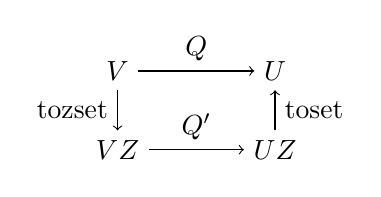
\begin{tikzpicture}
  \node[] (V) {$V$};
  \node[below of=V] (VZ) {$VZ$};
  \node[right of=V, node distance=2cm] (U) {$U$};
  \node[below of=U] (UZ) {$UZ$};
  \draw[->] (V) -- node (f) [above] {$Q$} (U);
  \draw[->] (V) --  node (s) [left] {tozset}(VZ);
  \draw[->] (VZ) -- node (f) [above] {$Q'$} (UZ);
  \draw[->] (UZ) -- node (d) [right] {toset} (U);
\end{tikzpicture}
\end{center}

The $\mbox{toset}$ and $\mbox{tozset}$ functions convert sets to \zrs and 
vice-versa:

$\mbox{toset}: \Z[A] \to 2^A$ is defined by $\mbox{toset}(m) \defn \cup_{x \in \distinct(m)} \{ x \}$.

$\mbox{tozset}: 2^A \to \Z[A]$ is defined by $\mbox{tozset}(s) \defn \sum_{x \in s} 1 \cdot x$.

All standard algebraic properties
of the relational operators can be used to optimize circuits
(they can even be applied to queries before building the circuits).

Notice that the use of the $\distinct$ operator allows DBSP to model
the \emph{full relational algebra}, including difference (and not just the positive
fragment).  Most of the operators that appear in the circuits in
Table~\ref{tab:relational} are linear, and thus have very efficient
incremental versions.  A notable exception is $\distinct$.  While we
show below that $\distinct$ can be computed efficiently incrementally,
it does have an important cost in terms of memory, so we try to 
minimize its use.  For this we can use a pair of optimizations:

\begin{proposition}\label{prop-distinct-delay}
Let Q be one of the following \zrs operators: filtering $\sigma$,
join $\bowtie$, or Cartesian product $\times$.
Then we have $\forall i \in \Z[I], \ispositive(i) \Rightarrow Q(\distinct(i)) = \distinct(Q(i))$.
\end{proposition}

\begin{comment}
\noindent
\begin{tabular}{m{3.5cm}m{.5cm}m{3.5cm}}
\begin{tikzpicture}[auto,>=latex]
  \node[] (input) {$i$};
  \node[block, right of=input, node distance=1.1cm] (distinct) {$\distinct$};
  \node[block, right of=distinct, node distance=1.2cm] (q) {$Q$};
  \node[right of=q] (output)  {$o$};
  \draw[->] (input) -- (distinct);
  \draw[->] (distinct) -- (q);
  \draw[->] (q) -- (output);
\end{tikzpicture}
&
$\cong$
&
\begin{tikzpicture}[auto,>=latex]
  \node[] (input) {$i$};
  \node[block, right of=input] (q) {$Q$};
  \node[block, right of=q, node distance=1.2cm] (distinct1) {$\distinct$};
  \node[right of=distinct1, node distance=1.2cm] (output)  {$o$};
  \draw[->] (input) -- (q);
  \draw[->] (q) -- (distinct1);
  \draw[->] (distinct1) -- (output);
\end{tikzpicture}
\end{tabular}
\end{comment}

This rule allows us to delay the application of $\distinct$.

\begin{proposition}\label{prop-distinct-once}
Let Q be one of the following \zrs operators: filtering $\sigma$,
projection $\pi$, selection (map($f$)), addition $+$, join $\bowtie$, or
Cartesian product $\times$.
Then we have $\forall i \in \Z[I], \ispositive(i) \Rightarrow \distinct(Q(\distinct(i))) = \distinct(Q(i))$.
\end{proposition}

This is Proposition 6.13 in~\cite{green-tcs11}.

\begin{comment}
\noindent
\begin{tabular}{m{6.5cm}m{.5cm}}
\begin{tikzpicture}[auto,>=latex]
  \node[] (input) {$i$};
  \node[block, right of=input, node distance=1.5cm] (distinct) {$\distinct$};
  \node[block, right of=distinct, node distance=1.5cm] (q) {$Q$};
  \node[block, right of=q, node distance=1.5cm] (distinct1) {$\distinct$};
  \node[right of=distinct1, node distance=1.5cm] (output)  {$o$};
  \draw[->] (input) -- (distinct);
  \draw[->] (distinct) -- (q);
  \draw[->] (q) -- (distinct1);
  \draw[->] (distinct1) -- (output);
\end{tikzpicture}
&
$\cong$ \\
\begin{tikzpicture}[auto,>=latex]
  \node[] (input) {$i$};
  \node[block, right of=input] (q) {$Q$};
  \node[block, right of=q, node distance=1.5cm] (distinct1) {$\distinct$};
  \node[right of=distinct1, node distance=1.5cm] (output)  {$o$};
  \draw[->] (input) -- (q);
  \draw[->] (q) -- (distinct1);
  \draw[->] (distinct1) -- (output);
\end{tikzpicture}
\end{tabular}
\end{comment}

These properties allow us to ``consolidate'' distinct operators by performing
one $\distinct$ at the end of a chain of computations.

Finally, the next proposition shows that the incremental of $\distinct$
can be computed with work proportional to the size of the input change.

\begin{proposition}\label{prop-inc_distinct}
The following circuit implements $\inc{(\lift{\distinct})}$:
\begin{tabular}{m{3.5cm}m{.5cm}m{6cm}}
\begin{tikzpicture}[auto,node distance=1.5cm,>=latex]
    \node[] (input) {$d$};
    \node[block, right of=input] (d) {$\inc{(\lift{\distinct})}$};
    \node[right of=d] (output) {$o$};
    \draw[->] (input) -- (d);
    \draw[->] (d) -- (output);
\end{tikzpicture} &
$\cong$ &
\begin{tikzpicture}[>=latex]
    \node[] (input) {$d$};
    \node[block, right of=input] (I) {$\I$};
    \node[block, right of=I] (z) {$\zm$};
    \node[block, below of=z, node distance=.8cm] (H) {$\lift{H}$};
    \node[right of=H] (output) {$o$};
    \draw[->] (input) -- node (mid) {} (I);
    \draw[->] (I) -- (z);
    \draw[->] (mid.center) |- (H);
    \draw[->] (z) -- node (i) [right] {$i$} (H);
    \draw[->] (H) -- (output);
\end{tikzpicture}
\end{tabular}

\noindent where $H: \Z[A] \times \Z[A] \to \Z[A]$ is defined as:
$$
H(i, d)[x] \defn 
\begin{cases}
-1 & \mbox{if } i[x] > 0 \mbox{ and } (i + d)[x] \leq 0 \\
1  & \mbox{if } i[x] \leq 0 \mbox{ and } (i + d)[x] > 0 \\
0  & \mbox{otherwise} \\
\end{cases}
$$
\end{proposition}

The function $H$ detects whether the multiplicity of an element in the 
input set $i$ when adding change $d$ is changing from negative to
positive or vice-versa.  Notice that only multiplicities of the elements
that appear in the change $d$ can change from input to output, so the
work needed to compute both $H$ is bounded by the size of $d$ and not $i$.

\subsection{Incremental view maintenance}

Let us consider a relational query $Q$ 
defining a view.  To create a circuit that maintains incrementally the view defined by $Q$
we apply the following mechanical steps; this algorithm is deterministic
and its running time is proportional to the complexity 
of the query (number of operators in the query):

\begin{algorithm}[incremental view maintenance]\label{algorithm-inc}\quad
\begin{enumerate}[nosep, leftmargin=\parindent]
    \item Translate $Q$ into a circuit using the rules in Table~\ref{tab:relational}.
    \item Apply $\distinct$ consolidation until convergence.
    \item Lift the whole circuit, by applying Proposition~\ref{prop:distributivity},
    converting it to a circuit operating on streams.
    \item Incrementalize the whole circuit ``surrounding'' it with $\I$ and $\D$.
    \item Apply the chain rule and other properties of the $\inc{\cdot}$ operator
    from Proposition~\ref{prop-inc-properties} recursively on the query structure
    to optimize the incremental implementation.  
\end{enumerate}
\end{algorithm}

Step (3) yields a circuit that consumes a stream of complete database snapshots and outputs a 
stream of complete view snapshots. Step (4) yields a circuit that consumes a stream of changes
to the database and outputs a stream of view changes; however, the internal operation of the 
circuit is non-incremental, as it computes on the complete state of the database reconstructed
by the integration operator.  Step (5) incrementalizes the internals of the circuit by rewriting 
it to compute on changes, avoiding integration when possible (see \secref{sec:incremental}).  

\subsection{Example}\label{sec:relational-example}

In this section we apply the incremental view maintenance algorithm to a concrete
query.  Let us consider the following query:

\begin{lstlisting}[language=SQL]
CREATE VIEW v AS
SELECT DISTINCT t1.x, t2.y FROM (
     SELECT t1.x, t1.id 
     FROM t 
     WHERE t.a > 2 
) t1  
JOIN (
     SELECT t2.id, t2.y
     FROM r 
     WHERE r.s > 5 
) t2 ON t1.id = t2.id
\end{lstlisting}

Step 1: First we create a \dbsp circuit to represent this query using the
translation rules from Table~\ref{tab:relational}:

\noindent
\begin{tikzpicture}[node distance=1.2cm,>=latex]
    \node[] (t1) {\code{t1}};
    \node[block, right of=t1, node distance=.9cm] (s1) {$\sigma_{a > 2}$};
    \node[block, right of=s1] (d1) {$\distinct$};
    \node[block, right of=d1] (p1) {$\pi_{x, d}$};
    \node[block, right of=p1] (d11) {$\distinct$};
    \node[below of=t1, node distance=1cm] (t2) {\code{t2}};
    \node[block, right of=t2, node distance=.9cm] (s2) {$\sigma_{s > 5}$};
    \node[block, right of=s2] (d2) {$\distinct$};
    \node[block, right of=d2] (p2) {$\pi_{y, id}$};
    \node[block, right of=p2] (d21) {$\distinct$};
    \node[below of=d11, node distance=.5cm] (mid) {};
    \node[block, right of=mid, node distance=.8cm] (j) {$\bowtie_{id = id}$};
    \node[block, right of=j] (p) {$\pi_{x, y}$};
    \node[block, right of=p] (d) {$\distinct$};
    \node[right of=d, node distance=.9cm] (V) {\code{V}};
    \draw[->] (t1) -- (s1);
    \draw[->] (s1) -- (d1);
    \draw[->] (d1) -- (p1);
    \draw[->] (p1) -- (d11);
    \draw[->] (t2) -- (s2);
    \draw[->] (s2) -- (d2);
    \draw[->] (d2) -- (p2);
    \draw[->] (p2) -- (d21);
    \draw[->] (d11) -| (j);
    \draw[->] (d21) -| (j);
    \draw[->] (j) -- (p);
    \draw[->] (p) -- (d);
    \draw[->] (d) -- (V);
\end{tikzpicture}

Step 2: we apply the $\distinct$ optimization rules; first the rule from~\ref{prop-distinct-once}
gives us the following equivalent circuit:

\noindent
\begin{tikzpicture}[node distance=1.2cm,>=latex]
    \node[] (t1) {\code{t1}};
    \node[block, right of=t1, node distance=.9cm] (s1) {$\sigma_{a > 2}$};
    \node[block, right of=s1] (p1) {$\pi_{x, d}$};
    \node[block, right of=p1] (d11) {$\distinct$};
    \node[below of=t1, node distance=1cm] (t2) {\code{t2}};
    \node[block, right of=t2, node distance=.9cm] (s2) {$\sigma_{s > 5}$};
    \node[block, right of=s2] (p2) {$\pi_{y, id}$};
    \node[block, right of=p2] (d21) {$\distinct$};
    \node[below of=d11, node distance=.5cm] (mid) {};
    \node[block, right of=mid, node distance=.8cm] (j) {$\bowtie_{id = id}$};
    \node[block, right of=j] (p) {$\pi_{x, y}$};
    \node[block, right of=p] (d) {$\distinct$};
    \node[right of=d, node distance=.9cm] (V) {\code{V}};
    \draw[->] (t1) -- (s1);
    \draw[->] (s1) -- (p1);
    \draw[->] (p1) -- (d11);
    \draw[->] (t2) -- (s2);
    \draw[->] (s2) -- (p2);
    \draw[->] (p2) -- (d21);
    \draw[->] (d11) -| (j);
    \draw[->] (d21) -| (j);
    \draw[->] (j) -- (p);
    \draw[->] (p) -- (d);
    \draw[->] (d) -- (V);
\end{tikzpicture}

Applying the rule from~\ref{prop-distinct-delay} we get:

\noindent
\begin{tikzpicture}[node distance=1.2cm,>=latex]
    \node[] (t1) {\code{t1}};
    \node[block, right of=t1, node distance=.9cm] (s1) {$\sigma_{a > 2}$};
    \node[block, right of=s1] (p1) {$\pi_{x, d}$};
    \node[below of=t1, node distance=1cm] (t2) {\code{t2}};
    \node[block, right of=t2, node distance=.9cm] (s2) {$\sigma_{s > 5}$};
    \node[block, right of=s2] (p2) {$\pi_{y, id}$};
    \node[below of=p1, node distance=.5cm] (mid) {};
    \node[block, right of=mid, node distance=.8cm] (j) {$\bowtie_{id = id}$};
    \node[block, right of=j] (d0) {$\distinct$};
    \node[block, right of=d0] (p) {$\pi_{x, y}$};
    \node[block, right of=p] (d) {$\distinct$};
    \node[right of=d, node distance=.9cm] (V) {\code{V}};
    \draw[->] (t1) -- (s1);
    \draw[->] (s1) -- (p1);
    \draw[->] (t2) -- (s2);
    \draw[->] (s2) -- (p2);
    \draw[->] (p1) -| (j);
    \draw[->] (p2) -| (j);
    \draw[->] (j) -- (d0);
    \draw[->] (d0) -- (p);
    \draw[->] (p) -- (d);
    \draw[->] (d) -- (V);
\end{tikzpicture}

And applying again~\ref{prop-distinct-once} we get:

\noindent
\begin{tikzpicture}[node distance=1.2cm,>=latex]
    \node[] (t1) {\code{t1}};
    \node[block, right of=t1, node distance=.9cm] (s1) {$\sigma_{a > 2}$};
    \node[block, right of=s1] (p1) {$\pi_{x, d}$};
    \node[below of=t1, node distance=1cm] (t2) {\code{t2}};
    \node[block, right of=t2, node distance=.9cm] (s2) {$\sigma_{s > 5}$};
    \node[block, right of=s2] (p2) {$\pi_{y, id}$};
    \node[below of=p1, node distance=.5cm] (mid) {};
    \node[block, right of=mid, node distance=.8cm] (j) {$\bowtie_{id = id}$};
    \node[block, right of=j] (p) {$\pi_{x, y}$};
    \node[block, right of=p] (d) {$\distinct$};
    \node[right of=d, node distance=.9cm] (V) {\code{V}};
    \draw[->] (t1) -- (s1);
    \draw[->] (s1) -- (p1);
    \draw[->] (t2) -- (s2);
    \draw[->] (s2) -- (p2);
    \draw[->] (p1) -| (j);
    \draw[->] (p2) -| (j);
    \draw[->] (j) -- (p);
    \draw[->] (p) -- (d);
    \draw[->] (d) -- (V);
\end{tikzpicture}

Step 3: we lift the circuit using distributivity of composition over lifting; we
obtain a circuit that computes over streams, i.e., for each new input pair of relations
\code{t1} and \code{t2} it will produce an output view \code{V}:

\noindent
\begin{tikzpicture}[node distance=1.3cm,>=latex]
    \node[] (t1) {\code{t1}};
    \node[block, right of=t1, node distance=.9cm] (s1) {$\lift{\sigma_{a > 2}}$};
    \node[block, right of=s1] (p1) {$\lift{\pi_{x, d}}$};
    \node[below of=t1, node distance=1.2cm] (t2) {\code{t2}};
    \node[block, right of=t2, node distance=.9cm] (s2) {$\lift{\sigma_{s > 5}}$};
    \node[block, right of=s2] (p2) {$\lift{\pi_{y, id}}$};
    \node[below of=p1, node distance=.6cm] (mid) {};
    \node[block, right of=mid, node distance=.8cm] (j) {$\lift{\bowtie_{id = id}}$};
    \node[block, right of=j] (p) {$\lift{\pi_{x, y}}$};
    \node[block, right of=p] (d) {$\lift{\distinct}$};
    \node[right of=d] (V) {\code{V}};
    \draw[->] (t1) -- (s1);
    \draw[->] (s1) -- (p1);
    \draw[->] (t2) -- (s2);
    \draw[->] (s2) -- (p2);
    \draw[->] (p1) -| (j);
    \draw[->] (p2) -| (j);
    \draw[->] (j) -- (p);
    \draw[->] (p) -- (d);
    \draw[->] (d) -- (V);
\end{tikzpicture}

Step 4: incrementalize circuit, obtaining a circuit that computes over changes;
this circuit receives changes to relations \code{t1} and \code{t2} and for each
such change it produces the corresponding change in the output view \code{V}:

\noindent
\begin{tikzpicture}[node distance=1.3cm,>=latex]
    \node[] (t1) {$\Delta$\code{t1}};
    \node[block, right of=t1, node distance=.8cm] (I1) {$\I$};
    \node[block, right of=I1, node distance=.9cm] (s1) {$\lift{\sigma_{a > 2}}$};
    \node[block, right of=s1] (p1) {$\lift{\pi_{x, d}}$};
    \node[below of=t1, node distance=1.2cm] (t2) {$\Delta$\code{t2}};
    \node[block, right of=t2, node distance=.8cm] (I2) {$\I$};
    \node[block, right of=I2, node distance=.9cm] (s2) {$\lift{\sigma_{s > 5}}$};
    \node[block, right of=s2] (p2) {$\lift{\pi_{y, id}}$};
    \node[below of=p1, node distance=.6cm] (mid) {};
    \node[block, right of=mid, node distance=.6cm] (j) {$\lift{\bowtie_{id = id}}$};
    \node[block, right of=j] (p) {$\lift{\pi_{x, y}}$};
    \node[block, right of=p] (d) {$\lift{\distinct}$};
    \node[block, right of=d, node distance=1.1cm] (D) {$\D$};
    \node[right of=D, node distance=.7cm] (V) {$\Delta$\code{V}};
    \draw[->] (t1) -- (I1);
    \draw[->] (I1) -- (s1);
    \draw[->] (s1) -- (p1);
    \draw[->] (t2) -- (I2);
    \draw[->] (I2) -- (s2);
    \draw[->] (s2) -- (p2);
    \draw[->] (p1) -| (j);
    \draw[->] (p2) -| (j);
    \draw[->] (j) -- (p);
    \draw[->] (p) -- (d);
    \draw[->] (d) -- (D);
    \draw[->] (D) -- (V);
\end{tikzpicture}

Step 5: apply the chain rule to rewrite the circuit as a composition of incremental operators;

\noindent
\begin{tikzpicture}[node distance=1.6cm,>=latex]
    \node[] (t1) {$\Delta$\code{t1}};
    \node[block, right of=t1, node distance=1.2cm] (s1) {$\inc{(\lift{\sigma_{a > 2}})}$};
    \node[block, right of=s1] (p1) {$\inc{(\lift{\pi_{x, d}})}$};
    \node[below of=t1, node distance=1.2cm] (t2) {$\Delta$\code{t2}};
    \node[block, right of=t2, node distance=1.2cm] (s2) {$\inc{(\lift{\sigma_{s > 5}})}$};
    \node[block, right of=s2] (p2) {$\inc{(\lift{\pi_{y, id}})}$};
    \node[below of=p1, node distance=.6cm] (mid) {};
    \node[block, right of=mid, node distance=.8cm] (j) {$\inc{(\lift{\bowtie_{id = id}})}$};
    \node[block, right of=j] (p) {$\inc{(\lift{\pi_{x, y}})}$};
    \node[block, right of=p] (d) {$\inc{(\lift{\distinct})}$};
    \node[right of=d, node distance=1.2cm] (V) {$\Delta$\code{V}};.8
    \draw[->] (t1) -- (s1);
    \draw[->] (s1) -- (p1);
    \draw[->] (t2) -- (s2);
    \draw[->] (s2) -- (p2);
    \draw[->] (p1) -| (j);
    \draw[->] (p2) -| (j);
    \draw[->] (j) -- (p);
    \draw[->] (p) -- (d);
    \draw[->] (d) -- (V);
\end{tikzpicture}

Use the linearity of $\sigma$ and $\pi$ to simplify this circuit:

\noindent
\begin{tikzpicture}[node distance=1.6cm,>=latex]
    \node[] (t1) {$\Delta$\code{t1}};
    \node[block, right of=t1, node distance=1cm] (s1) {$\lift{\sigma_{a > 2}}$};
    \node[block, right of=s1] (p1) {$\lift{\pi_{x, d}}$};
    \node[below of=t1, node distance=1.2cm] (t2) {$\Delta$\code{t2}};
    \node[block, right of=t2, node distance=1cm] (s2) {$\lift{\sigma_{s > 5}}$};
    \node[block, right of=s2] (p2) {$\lift{\pi_{y, id}}$};
    \node[below of=p1, node distance=.6cm] (mid) {};
    \node[block, right of=mid, node distance=.8cm] (j) {$\inc{(\lift{\bowtie_{id = id}})}$};
    \node[block, right of=j] (p) {$\lift{\pi_{x, y}}$};
    \node[block, right of=p] (d) {$\inc{(\lift{\distinct})}$};
    \node[right of=d, node distance=1.3cm] (V) {$\Delta$\code{V}};.8
    \draw[->] (t1) -- (s1);
    \draw[->] (s1) -- (p1);
    \draw[->] (t2) -- (s2);
    \draw[->] (s2) -- (p2);
    \draw[->] (p1) -| (j);
    \draw[->] (p2) -| (j);
    \draw[->] (j) -- (p);
    \draw[->] (p) -- (d);
    \draw[->] (d) -- (V);
\end{tikzpicture}

Finally, replace the incremental join using the formula for bilinear operators 
(Theorem~\ref{bilinear}),
and the incremental $\distinct$ (Proposition~\ref{prop-inc_distinct}),
obtaining the circuit from Figure~\ref{fig:relational-example}.

\begin{figure*}[h]
\begin{tikzpicture}[node distance=1.5cm,>=latex]
    \node[] (t1) {$\Delta$\code{t1}};
    \node[block, right of=t1, node distance=1cm] (s1) {$\lift{\sigma_{a > 2}}$};
    \node[block, right of=s1] (p1) {$\lift{\pi_{x, d}}$};
    \node[below of=t1, node distance=1.6cm] (t2) {$\Delta$\code{t2}};
    \node[block, right of=t2, node distance=1cm] (s2) {$\lift{\sigma_{s > 5}}$};
    \node[block, right of=s2] (p2) {$\lift{\pi_{y, id}}$};
    
    % join expansion
      \node[block, right of=p1, node distance=1cm] (jI1) {$\I$};
      \node[block, below of=p1, node distance=.8cm] (ab) {$\lift\bowtie_{id=id}$};
      \node[block, right of=p2, node distance=1cm] (jI2) {$\I$};
      \draw[->] (p1) -- (jI1);
      \draw[->] (p2) -- (jI2);
      \node[block, right of=jI1, node distance=.8cm] (ZI1) {$\zm$};
      \node[block, right of=jI2, node distance=.8cm] (ZI2) {$\zm$};
      \draw[->] (jI1) -- (ZI1);
      \draw[->] (jI2) -- (ZI2);
      \node[block, right of=ZI1] (DI1) {$\lift\bowtie_{id=id}$};
      \node[block, right of=ZI2] (DI2) {$\lift\bowtie_{id=id}$};
      \draw[->] (ZI1) -- (DI1);
      \draw[->] (ZI2) -- (DI2);
      \node[block, circle, below of=DI1, inner sep=0cm, node distance=.8cm] (sum) {$+$};
      \draw[->] (ab) -- (sum);
      \draw[->] (DI1) -- (sum);
      \draw[->] (DI2) -- (sum);
      \draw[->] (p1) -- (ab);
      \draw[->] (p2) -- (ab);
      \draw[->] (p1) -- (DI2);
      \draw[->] (p2) -- (DI1);
    
    \node[block, right of=sum] (p) {$\lift{\pi_{x, y}}$};
    \draw[->] (sum) -- (p);
    \node[block, right of=p] (Id) {$\I$};
    \node[block, right of=Id, node distance=.8cm] (zd) {$\zm$};
    \node[block, below of=zd, node distance=.8cm] (H) {$\lift{H}$};
    \node[right of=H, node distance=1.3cm] (V) {$\Delta$\code{V}};.8
    \draw[->] (t1) -- (s1);
    \draw[->] (s1) -- (p1);
    \draw[->] (t2) -- (s2);
    \draw[->] (s2) -- (p2);
    \draw[->] (p) -- node (tapp) {} (Id);
    \draw[->] (Id) -- (zd);
    \draw[->] (zd) -- (H);
    \draw[->] (tapp.center) |- (H);
    \draw[->] (H) -- (V);
\end{tikzpicture}
\caption{Final version of the incremental query circuit from 
\refsec{sec:relational-example}\label{fig:relational-example}.}
\end{figure*}

Notice that the resulting circuit contains three integration operations: two from
the join, and one from the $\distinct$.  It also contains three join operators.
However, the work performed by each operator
for each new input is proportional to the size of change, as we argue in the following section.

\subsection{Complexity}

Incremental circuits are efficient.  The work performed (and the memory used) by a circuit
is the sum of the work performed (and memory used) by its operators.
We argue that each operator in the incremental version of a circuit is efficient.

For incrementalized circuits the input stream of each operator contains \emph{changes} in
its input relations.  Denote $C[t] \defn \norm{s[t]}$ the \defined{size}
of the value of stream $s$ of changes at time $t$, and $R[t] \defn
\norm{\I(s)[t]}$ the size of the relation produced by integrating all changes in
$s$.  An unoptimized incremental operator $\inc{Q} = \D \circ Q \circ \I$
evaluates query $Q$ on the integration of its input streams; hence its time
complexity  is the same as that of the non-incremental operator, a function of
$R[t]$.  In addition, because of the $\I$ and $\D$ operators, it uses $O(R[t])$ memory.

The optimizations described in \secref{sec:incremental} reduce the
reduce the time complexity of an operator to be a function of $C[t]$.  Assuming $C[t] \ll
R[t]$, this translates to major performance improvements in practice.  For
example, Theorem~\ref{linear}, allows evaluating $\inc{T}$, where $T$ is a
linear operator, in time $O(C[t])$.  Interestingly, while the $\I$
operator uses $O(R[t])$ memory, it can be evaluated in $O(C[t])$ time, because 
all values that appear in the output at time $t$ must be present in
current input change for time $t$.  Similarly, while the $\distinct$ operator is not
linear, $\inc{(\lift{\distinct})}$ can also be evaluated in $O(C[t])$ according to
Proposition~\ref{prop-inc_distinct}.  Bilinear operators, including join, can be
evaluated in time proportional to the product of the sizes of their input
changes $O(C[t]^2)$ (Theorem~\ref{bilinear}).  

The space complexity of linear operators is 0 (zero), since they store no
data persistently.  The space complexity of $\inc{(\lift{\distinct})}$ and 
join is $O(R[t])$.